
\documentclass[12pt]{article}

% Layout.
\usepackage[top=1in, bottom=0.75in, left=1in, right=1in, headheight=1in, headsep=6pt]{geometry}

% Fonts.
\usepackage{mathptmx}
\usepackage[scaled=0.86]{helvet}
\renewcommand{\emph}[1]{\textsf{\textbf{#1}}}

% TiKZ.
\usepackage{tikz, pgfplots}
\usetikzlibrary{calc}
\pgfplotsset{compat = newest}
 
\pgfplotsset{my style/.append style={axis x line=middle, axis y line=
middle, xlabel={$x$}, ylabel={$y$}, axis equal }}

% Misc packages.
\usepackage{amsmath,amssymb,latexsym}
\usepackage{graphicx}
\usepackage{array}
\usepackage{xcolor}
\usepackage{multicol}

% Commands to set various header/footer components.
\makeatletter
\def\doctitle#1{\gdef\@doctitle{#1}}
\doctitle{Use {\tt\textbackslash doctitle\{MY LABEL\}}.}
\def\docdate#1{\gdef\@docdate{#1}}
\docdate{Use {\tt\textbackslash docdate\{MY DATE\}}.}
\def\doccourse#1{\gdef\@doccourse{#1}}
\let\@doccourse\@empty
\def\docscoring#1{\gdef\@docscoring{#1}}
\let\@docscoring\@empty
\def\docversion#1{\gdef\@docversion{#1}}
\let\@docversion\@empty
\makeatother

% Headers and footers layout.
\makeatletter
\usepackage{fancyhdr}
\pagestyle{fancy}
\fancyhf{} % Clears all headers/footers.
\lhead{\baselineskip 30pt
%\emph{\@doctitle\hfill\@docdate}
\emph{\@docdate\hfill\@doctitle}
\ifnum \value{page} > 1\relax\else\\
\emph{Name: \rule{3.5in}{1pt}\hfill \@docscoring}\fi}
\rfoot{\emph{\@docversion}}
\lfoot{\emph{\@doccourse}}
\cfoot{\emph{\thepage}}
\renewcommand{\headrulewidth}{0pt}%
\makeatother

% Paragraph spacing
\parindent 0pt
\parskip 6pt plus 1pt

% A problem is a section-like command. Use \problem{5} to
% start a problem worth 5 points.
\newcounter{probcount}
\newcounter{subprobcount}
\setcounter{probcount}{0}
\newcommand{\problem}[1]{%
\par
\addvspace{4pt}%
\setcounter{subprobcount}{0}%
\stepcounter{probcount}%
%\makebox[0pt][r]{\emph{\arabic{probcount}.}\hskip1ex}\emph{[#1 points]}\hskip1ex}
\makebox[0pt][r]{\emph{\arabic{probcount}.}\hskip1ex}\emph{[#1 \ifnum1=0#1\relax point\else points\fi]}\hskip1ex}
%\textbf{(#1 \ifnum1=0#1\relax thing\else things\fi
\newcommand{\thesubproblem}{\emph{\alph{subprobcount}.}}

% Subproblems are an enumerate-like environment with a consistent
% numbering scheme. 
% Use \begin{subproblems}\item...\item...\end{subproblems}
\newenvironment{subproblems}{%
\begin{enumerate}%
\setcounter{enumi}{\value{subprobcount}}%
\renewcommand{\theenumi}{\emph{\alph{enumi}}}}%
{\setcounter{subprobcount}{\value{enumi}}\end{enumerate}}

% Blanks for answers in normal and math mode.
\newcommand{\blank}[1]{\rule{#1}{0.75pt}}
\newcommand{\mblank}[1]{\underline{\hspace{#1}}}
\def\emptybox(#1,#2){\framebox{\parbox[c][#2]{#1}{\rule{0pt}{0pt}}}}

% Misc.
\renewcommand{\d}{\displaystyle}
\newcommand{\ds}{\displaystyle}
\def\bc{\begin{center}}
\def\ec{\end{center}}
\def\be{\begin{enumerate}}
\def\ee{\end{enumerate}}

\newcommand{\ans}{\rule{2 in}{.5pt}}
\newcommand{\bigans}[1]{\rule{#1 in}{.5pt}}

\doctitle{Math F251X: Quiz 1}
\docdate{Fall 2024}
\doccourse{UAF Calculus I}
\docversion{v-1}
\docscoring{\blank{0.8in} / 40}
\begin{document}
%\textbf{Please circle your instructor's name:} \hfill Leah Berman  \hfill   Jill Faudree\\

There are 16 questions worth 40 points on this quiz. No aids (book, calculator, etc.)
are permitted.  {\bf Show all work for full credit.} Give \emph{exact} numerical answers such as $\sqrt{7}$ or $\frac{5}{\pi}.$

%%%Page 1 ALGEBRA
\begin{center}\textbf{Algebra} \end{center}
%Problem
\problem{2} Simplify each expression below.
	\begin{subproblems}
	\item Write the expression $\large{\displaystyle{\frac{(xyz)^3}{x^4y^{-2}z}}}$ in the form $x^ay^bz^c$. That is, write the expression with all terms in the numerator. 	\\
\vfill
\quad \hspace{4in} \underline{\hspace{2in}}
	\item Cancel any common factors in both the numerator and denominator for the expression $\large{\displaystyle{\frac{2xy^2+4y^3}{3x^2+6xy}}}.$\\
\vfill
\quad \hspace{4in} \underline{\hspace{2in}}
	\end{subproblems}

\problem{2} Solve the following equations for $x$ (giving exact answers).
	\begin{subproblems}
	\item   $5^x+1=12.$\\
\vfill
\quad \hspace{4in} \underline{\hspace{2in}}
	\item  $\displaystyle {\ln(x+3)}=\frac{1}{2}.$\\
\vfill
\quad \hspace{4in} \underline{\hspace{2in}}
	\end{subproblems}

%%%Problem
\problem{3} Solve the inequality $x^2 < 4$ for $x.$ Write your answer in interval notation.\\
\vfill
\quad \hspace{4in} \underline{\hspace{2in}}

\newpage 
%%%Page 2 Geo + Trig
\begin{center}\textbf{Geometry and Trigonometry} \end{center}

%%%Problem
\problem{2} A circular field has an area of 83 square feet. Determine its radius. Include units with your answer. \\
\vfill
\quad \hspace{4in} \underline{\hspace{2in}}

%%%Problem
\problem{2} Write an equation of the line between the points $(-3,2)$ and $(4,0).$ \\

\vfill

\quad \hspace{4in} \underline{\hspace{2in}}\\

%%%Problem
\problem{1} Evaluate $\sin(5 \pi/6)$ exactly.\\
\vfill
\quad \hspace{4in} \underline{\hspace{2in}}

%%%Problem
\problem{2} Solve the equation $\cos(x)=0$ on the interval $0 \leq x < 2\pi.$ Give your answer in \emph{radians}.\\
\vfill
\quad \hspace{4in} \underline{\hspace{2in}}

%%%Problem
\problem{2} In the right triangle below, $\sin(\theta) = \frac{1}{4}.$ Determine $\tan(\theta).$ 

\begin{multicols}{2}

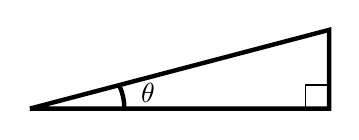
\begin{tikzpicture}
\draw[ultra thick] (0,0)--(3.8,0)--(3.8,1)--(0,0);
\node at (1.5,0.2){$\theta$};
\draw[ultra thick] (1.2,0) arc (0:24:0.7);
\draw (3.5,0)--(3.5,0.3)--(3.8,0.3);
\end{tikzpicture}

\columnbreak

\quad\\

\vspace{.4in}

$\tan(\theta)=$ \underline{\hspace{2in}}

\end{multicols}




\newpage

%%%Page 3 FUNCTIONS
\begin{center}\textbf{Functions} \end{center}
%%%Problem
\problem{2} Determine the domain and range of $f(x)=3+\sqrt{x}.$ Write your answer in interval notation. \\

\vfill

 domain:  \underline{\hspace{2in}} \hfill range:  \underline{\hspace{2in}}\\

%%%Problem
\problem{2} For $f(x)=x - x^2,$ find $f(a+2).$ Simplify your answer by multiplying out and collecting like terms.\\
\vfill
\quad \hspace{4in} \underline{\hspace{2in}}

%%%Problem
\problem{2} Use the piecewise defined function $\displaystyle f(x)=\begin{cases} x+1 & x \leq 0 \\ \frac{1}{x}& x>0 \end{cases}. $\\
	\begin{subproblems}
	\item Find $f(-2.4).$ \hfill \underline{\hspace{2in}}\\
	\vfill
	\item Determine $x$ such that $f(x)=4.$ \hfill \underline{\hspace{2in}}\\
	\vfill
	\end{subproblems}
%%%Problem
\problem{3} Use the graph of $f(x)$ below to answer the questions.\\

\begin{minipage}{.4\textwidth}
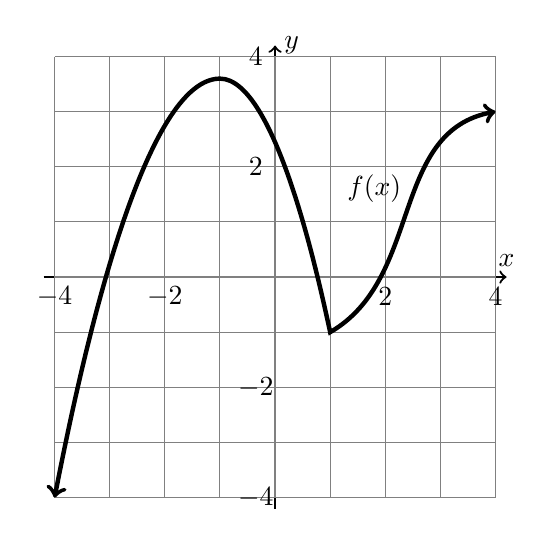
\begin{tikzpicture}[scale=.7]
%axes
\draw[thick, ->] (-4.2,0) -- (4.2,0);\draw[thick, ->] (0,-4.2) -- (0,4.2);
%labels for axes
\node at (4.2,.3){$x$}; \node at (.3,4.2){$y$};
%grid for axes
\foreach \i in {-4,-3,...,4}{
	\draw[gray] (-4,\i) -- (4,\i); \draw[gray] (\i,-4) -- (\i,4);

	}
\foreach \i in {-4,-2,2,4}{
	\node at (\i,-.35){$\i$};
	\node at (-.35,\i){$\i$};
	}
%location of label f(x)
\node at (1.8, 1.6) {$f(x)$};
%graphs of bendy + parabola
\draw[ultra thick, <->] (4, 3) to[in = 30, out = 190] (1,-1) parabola bend (-1, 3.6) (-4,-4);
\end{tikzpicture}
\end{minipage}
\begin{minipage}{.6\textwidth}
	\begin{subproblems}
	\item {\bf Estimate} $f(3)$. \hfill \ans 
	\vspace{12 pt}
	\item {\bf Estimate} an $x$-value such that $f(x)=-2.$ 
	\vspace{12 pt}
	
	\hfill \ans
	
	\item On the interval from $x=1$ to $x=3$, is $f(x)$ increasing, decreasing, or constant?
	\vspace{12 pt}
	
	\hfill \ans
	\end{subproblems}
\end{minipage}	
\newpage
%%%PAGE 4

\textbf{Graphing}\\
For problems 13-16, graph each function on the axes provided. Draw any asymptotes with dashed lines. Fill in the blanks identifying any $x$- or $y$-intercepts and the \emph{equations} of any asymptotes. Write \emph{none} if no intercepts or asymptotes exist.\\

%%%Problem
\problem{4}  $f(x)= 4-x^2.$ \\

\begin{multicols}{2}
\begin{tikzpicture}[scale=0.7]
\draw[->](-4,0)--(4,0);\draw[->](0,-4)--(0,4);
\end{tikzpicture}
\columnbreak

 $x$ intercepts:  \underline{\hspace{2in}} \\ 
 
 $y$-intercepts:  \underline{\hspace{2in}} \\ 
 
 asymptote(s):  \underline{\hspace{2in}}\\
\end{multicols}
\vfill

%%%Problem
\problem{4} $f(x)=e^{x}+2$\\
\begin{multicols}{2}
\begin{tikzpicture}[scale=0.7]
\draw[->](-4,0)--(4,0);\draw[->](0,-3.5)--(0,4);
\end{tikzpicture}

\columnbreak

$x$ intercepts:  \underline{\hspace{2in}}\\

$y$-intercepts:  \underline{\hspace{2in}}\\

asymptote(s):  \underline{\hspace{2in}}\\


\end{multicols}
\vfill
\newpage
%page 5
%%%Problem
\problem{4} $f(x)=\ln(x-3)$\\
\begin{multicols}{2}
\begin{tikzpicture}[scale=0.7]
\draw[->](-4,0)--(4,0);\draw[->](0,-4)--(0,3.5);
\end{tikzpicture}

\columnbreak

$x$ intercepts:  \underline{\hspace{2in}}\\

$y$-intercepts:  \underline{\hspace{2in}}\\

asymptote(s):  \underline{\hspace{2in}}\\

\end{multicols}

%%%Problem
\problem{4} $f(x)=-\cos(x)$ on the interval $0 \leq x \leq 3\pi.$ \\
\vfill
%\begin{multicols}{2}
\begin{tikzpicture}[scale=0.7]
\draw[->](-1,0)--(20,0);\draw[->](0,-4)--(0,4);
\end{tikzpicture}

%\columnbreak
\vfill
$x$ intercepts:  \underline{\hspace{2in}}\\

$y$-intercepts:  \underline{\hspace{2in}}\\

asymptote(s):  \underline{\hspace{2in}}\\

%\end{multicols}
\vfill

\end{document}